\chapter{Financial Project Planning}
\section{Budgeting}
\subsection{What is budgeting?}
Budgeting involves examining:
\begin{itemize}
    \item Estimated revenues
    \item Estimated expenditures
\end{itemize}
over a specific period in the future, to determine a prediction of future company performance.
\subsection{What information is used for budgeting?}
\begin{enumerate}
    \item Accounting records
    \item Other sources within the company e.g. engineering / sales / production teams
    \item Sources outside the company e.g. published information, personal contacts
    \item Research and development
\end{enumerate}
in decreasing order of importance (approximately).
\subsection{Types of budget}
\begin{enumerate}
    \item Master budget: aggregation of lower-level budgets
    \item Operating budget: ``projected income statement''
    \item Cash budget: ``cash flow forecast''
    \item Capital budget: ``projected balance sheet''
    \item Labour budget: ``Staffing forecast''
    \item Static budget: fixed revenue and expenses
\end{enumerate}
\subsection{Example 1: Operating budget}
Deere Consulting Ltd. has the following income statement for 2021:
\begin{table}[H]
    \centering
    \begin{tabular}{@{}lr@{}}
        \toprule
        \textbf{Revenue}            & \textbf{\pounds (,000)} \\
        \midrule
        Sales                       & 25,323                  \\
        Cost of goods sold          & 18,582                  \\
        \midrule
        Gross profit                & 6,741                   \\
        \midrule
        \textbf{Operating expenses} &                         \\
        \midrule
        Total operating expenses    & 5,223                   \\
        \midrule
        Net income                  & 1,280                   \\
        \bottomrule
    \end{tabular}
    \caption{Deere Consulting Ltd. Income Statement. Year ended 31 December, 2021.}
\end{table}
Deere Consulting Ltd. has provided the following supplementary information to further assist with the budget:
\begin{itemize}
    \item Operating expenses are expected to increase to \pounds 5.62 million and sales are expected to increase proportionally
    \item The gross profit margin is expected to remain unchanged
\end{itemize}
Currently:
\begin{gather}
    \frac{\textrm{Sales}}{\textrm{Op. Ex}} = \frac{25323}{5223} = 4.85\\
    \textrm{Gross profit margin} = \frac{\textrm{Gross profit}}{\textrm{Sales}} = \frac{6741}{25323} = 26.6\%
\end{gather}
\begin{table}[H]
    \centering
    \begin{tabular}{@{}lr@{}}
        \toprule
        \textbf{Revenue}            & \textbf{\pounds (,000)} \\
        \midrule
        Sales                       & 27,257                  \\
        Cost of goods sold          & 20,007                  \\
        \midrule
        Gross profit                & 7,250                   \\
        \midrule
        \textbf{Operating expenses} &                         \\
        \midrule
        Total operating expenses    & 5,620                   \\
        \midrule
        Net income                  & 1,360                   \\
        \bottomrule
    \end{tabular}
    \caption{Deere Consulting Ltd. Income Statement. Year ended 31 December, 2022.}
\end{table}
\section{Cash flow forecast}
Cash flow forecasts are useful for clarifying the consequences of flows of money that occur at various times.
\begin{gather}
    \textrm{Net Cash Flow over time } t =\\
    \sum \textrm{Cash inflows in $t$} - \sum \textrm{Cash outflows in $t$}
\end{gather}
Cash flow forecasts are important because they form the basis of evaluating alternative projects.

Cash flow diagrams can be used to visualise flows of money that occur at various times.
\begin{figure}[H]
    \centering
    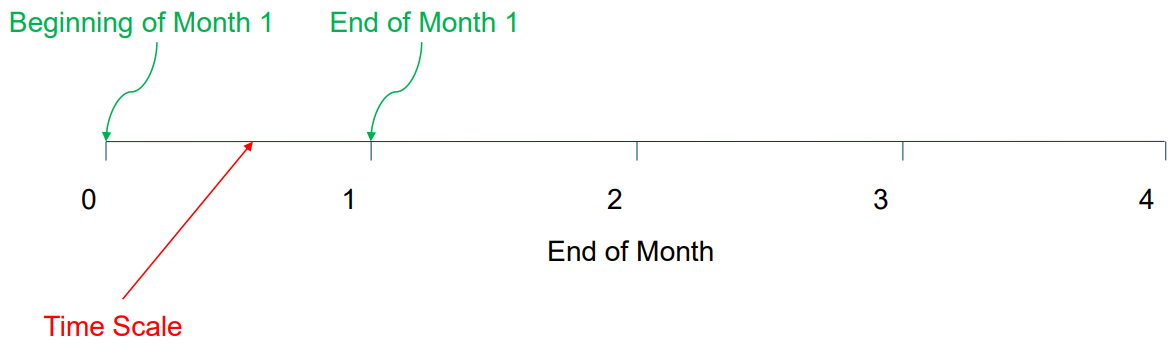
\includegraphics[width = 0.8\textwidth]{img/figure52.png}
    \caption{Cash flow forecast.}
\end{figure}
\begin{figure}[H]
    \centering
    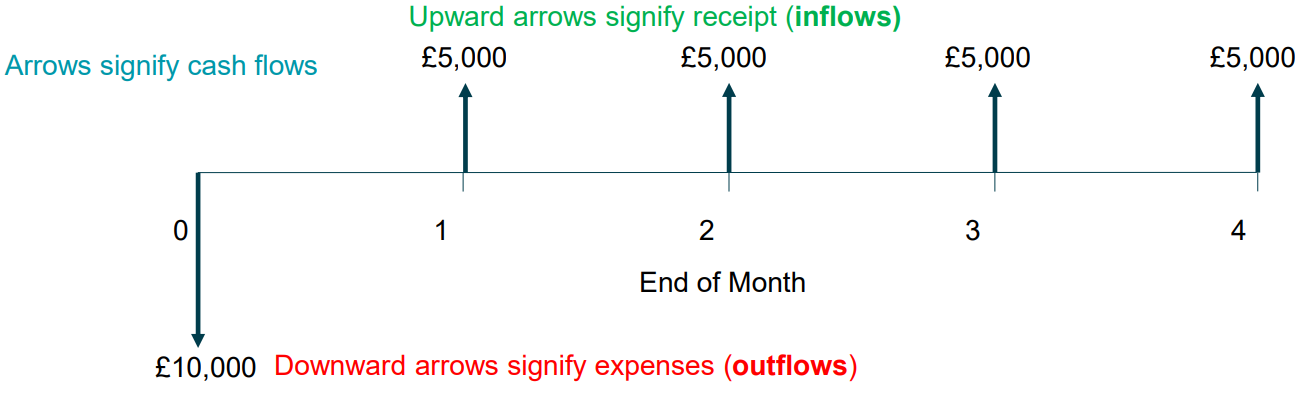
\includegraphics[width = 0.8\textwidth]{img/figure53.png}
    \caption{Cash flow forecast.}
\end{figure}
\subsection{Example 2}
Before evaluating the economic merits of a proposed investment, the ABC corporation insists that its engineers develop a cash-flow diagram of the proposal. An investment of \pounds 10,000 can be made that will produce uniform annual revenue of \pounds 5,310 for five years and then have a market (recovery) value of \pounds 2,000 at the EOY five. Annual expenses will be \pounds 3,000 at the end of each year for operating and maintaining the project.
\begin{quoting}
    Draw a cash-flow diagram for the five-year life of the project. Use the corporation's viewpoint
\end{quoting}
\begin{figure}[H]
    \centering
    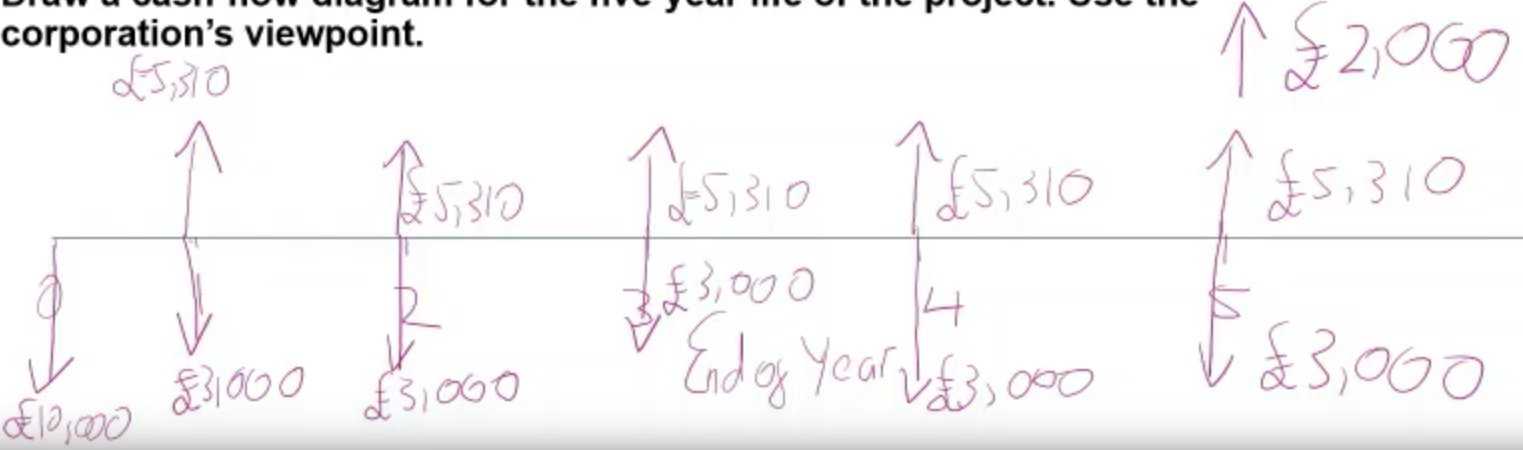
\includegraphics[width = 0.8\textwidth]{img/figure55.png}
    \caption{Cash flow diagram for ABC corporation.}
\end{figure}
So far, we have neglected the time value of money.
\begin{figure}[H]
    \centering
    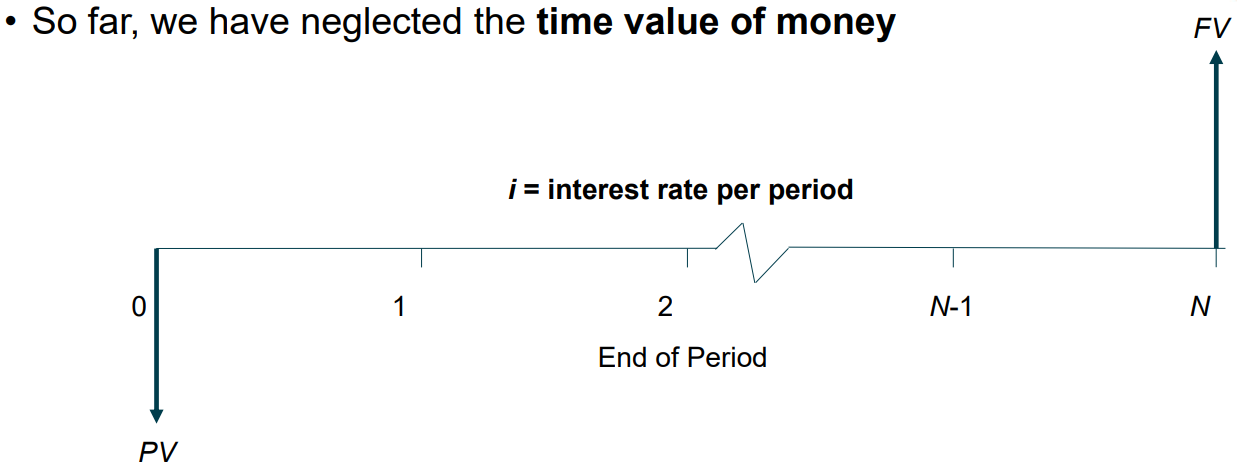
\includegraphics[width = 0.8\textwidth]{img/figure54.png}
    \caption{Time value of money in cash flow forecast.}
\end{figure}
\subsection{Time value of money}
Remember the formula for PV:
\begin{equation}
    PV = \frac{FV}{\left(1+i\right)^n}
\end{equation}
Present value (PV) of future value (FV) in $n$ periods, for an interest rate $i$.

Remember the formula for AV:
\begin{equation}
    AV = PV \frac{i\left(1 + i\right)^n}{\left(1+i\right)^n - 1}
\end{equation}
Value of a series of uniform (annual) receipts (AV) that occur at the end of periods 1 to $n$, given their present value (PV) and an interest rate $i$.
\subsection{Example 3}
A processing plant is considering the installation of a newly designed solar energy system that will power the majority of its energy operations, and sell \pounds 450,000 per year of surplus energy to the grid over its expected lifetime of 10 years. If the interest rate is 12\% per year, how much money can the plant afford to invest in the new boiler system?
\begin{figure}[H]
    \centering
    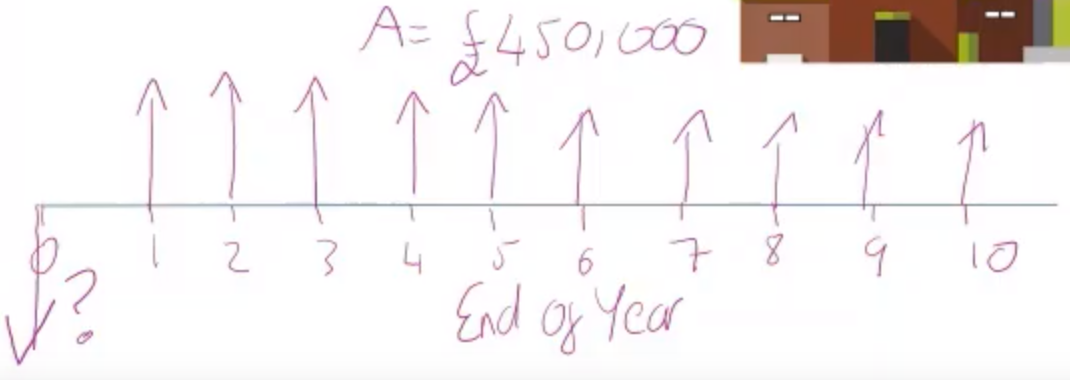
\includegraphics[width = 0.8\textwidth]{img/figure56.png}
    \caption{Cash flow diagram. Example 3.}
\end{figure}
\begin{gather}
    i = 0.12 \qquad n = 10\\
    PV = AV \frac{\left(1 + i\right)^n - 1}{i\left(1+i\right)^n}\\
    PV = 450000\times \frac{\left(1 + 0.12\right)^{10} - 1}{0.12\left(1+ 0.12\right)^{10}}\\
    PV = \pounds 2,542,600
\end{gather}
which is the upper limit on what the plant can afford to spend on the steam system.
\subsection{Example 4}
Automotive Engineering Ltd. is required to pay money into a compensatory fund, to cover damages caused by a company-related accident. The company will pay in \pounds 3 billion at the end of the third quarter of 2022 and another \pounds 2 billion in the fourth quarter of 2022. Twelve additional payments of \pounds 1.25 billion each quarter thereafter will result in a total of \pounds 20 billion having been paid into the fund. The interest rate is 3\% per quarter.
\begin{quoting}
    What will be the value of this payment stream at the beginning of the third quarter of 2022?
\end{quoting}
\begin{figure}[H]
    \centering
    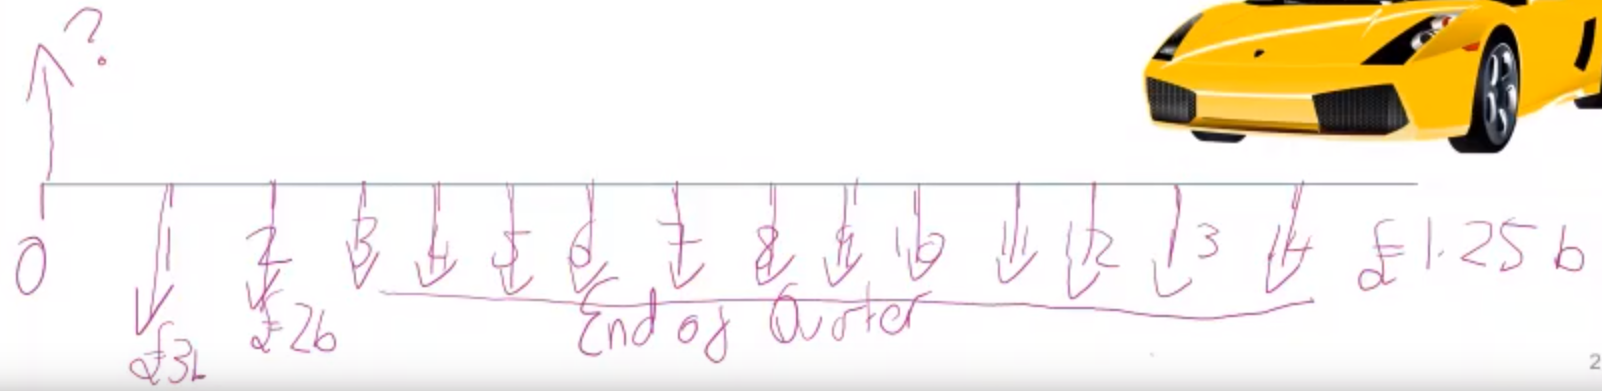
\includegraphics[width = 0.8\textwidth]{img/figure57.png}
    \caption{Cash flow diagram. Example 4.}
\end{figure}
PV of first end-of-quarter payment (\pounds 3 billion):
\begin{gather}
    \frac{3}{\left(1+0.03\right)^1} = \pounds 2.91\textrm{b}
\end{gather}
PV of second end-of-quarter payment (\pounds 2 billion):
\begin{gather}
    \frac{2}{\left(1+0.03\right)^2} = \pounds 1.89\textrm{b}
\end{gather}
FV of subsequent end-of-quarter payment (\pounds 1.25 billion):
\begin{gather}
    1.25\times \frac{\left(1+0.03\right)^{12}-1}{0.03\left(1+0.03\right)^{12}} = \pounds 12.44\textrm{b}
\end{gather}
PV of subsequent end-of-quarter payment (\pounds 1.25 billion):
\begin{gather}
    \frac{12.44}{\left(1+0.03\right)^2} = \pounds 11.73\textrm{b}
\end{gather}
PV of payment stream:
\begin{gather}
    2.91 + 1.89 + 11.73 = \pounds 16.53\textrm{b}
\end{gather}
\subsection{Cash flow forecast: table}
Cash flow tables are useful when the complexity of a situation makes it difficult to show all cash-flow amounts on a diagram. Cash flow tables can facilitate the analysis of different plans and designs. Cash flow tables clarify:
\begin{enumerate}
    \item The timing of cash flows
    \item The assumptions being made
    \item The amount of data available
\end{enumerate}
\subsection{Example 5}
CEGE Ltd. is renovating its office building and have identified two feasible alternatives for upgrading the heating, ventilation and air conditioning (HVAC) system. Either alternative A or alternative B must be implemented. The costs are as follows.
\begin{table}[H]
    \centering
    \begin{tabular}{@{}lr@{}}
        \toprule
        Equipment, labour and materials to rebuild & \pounds 18,000 \\
        Annual cost of electricity                 & \pounds 32,000 \\
        Annual maintenance expenses                & \pounds 2,400  \\
        Estimated market value (after eight years) & \pounds 2,000  \\
        \bottomrule
    \end{tabular}
    \caption{Alternative A: Rebuild (overhaul) the existing HVAC system.}
\end{table}
\begin{table}[H]
    \centering
    \begin{tabular}{@{}lr@{}}
        \toprule
        Equipment, labour and materials to rebuild     & \pounds 60,000 \\
        Annual cost of electricity                     & \pounds 9,000  \\
        Annual maintenance expenses                    & \pounds 16,000 \\
        Replacement of a major component in four years & \pounds 9,400  \\
        Estimated market value (after eight years)     & \pounds 8,000  \\
        \bottomrule
    \end{tabular}
    \caption{Alternative B: Install a new HVAC system that uses existing equipment.}
\end{table}
Assume that both alternatives will provide equivalent services over an eight-year period.
\begin{quoting}
    Use a cash flow table to tabulate the net cash flows for both alternatives.
\end{quoting}
\begin{quoting}
    Determine the annual net cash flow difference between the alternatives (B-A).
\end{quoting}
\begin{table}[H]
    \centering
    \begin{tabular}{@{}lllll@{}}
        \toprule
                    & \textbf{Alternative A}  & \textbf{Alternative B}  & \textbf{Difference} & \textbf{Cumulative}  \\
        End of year & Net cash flow (\pounds) & Net cash flow (\pounds) & B-A (\pounds)       & Difference (\pounds) \\
        \midrule
        0           & -18,000                 & -60,000                 & -42,000             & -42,000              \\
        1           & -34,400                 & -25000                  & 9,400               & -32,600              \\
        2           & -34,400                 & -25000                  & 9,400               & -23,200              \\
        3           & -34,400                 & -25000                  & 9,400               & -13,800              \\
        4           & -34,400                 & -34400                  & 0                   & -13,800              \\
        5           & -34,400                 & -25000                  & 9,400               & -4,400               \\
        6           & -34,400                 & -25000                  & 9,400               & 5,000                \\
        7           & -34,400                 & -25000                  & 9,400               & 14,400               \\
        8           & -32,400                 & -17000                  & 15,400              & 29,800               \\
        \midrule
        Total       & -291,200                & -261,400                &                     & 29,800               \\
        \bottomrule
    \end{tabular}
    \caption{Example 5 table.}
\end{table}
Some important notes:
\begin{itemize}
    \item Timing is everything
          \begin{itemize}
              \item When is money being received?
              \item When is money being paid?
          \end{itemize}
    \item Cash flows deal with expected actual receipts and payments
          \begin{itemize}
              \item Debtors and creditors (from the balance sheet) do not appear
          \end{itemize}
    \item Cash flow forecasts can act as an early warning system
          \begin{itemize}
              \item Can help identify the need for a loan or overdraft far in advance
          \end{itemize}
\end{itemize}
\section{S-curves}
Display cumulative data (costs, hours, quantities etc.) for a project.
\begin{figure}[H]
    \centering
    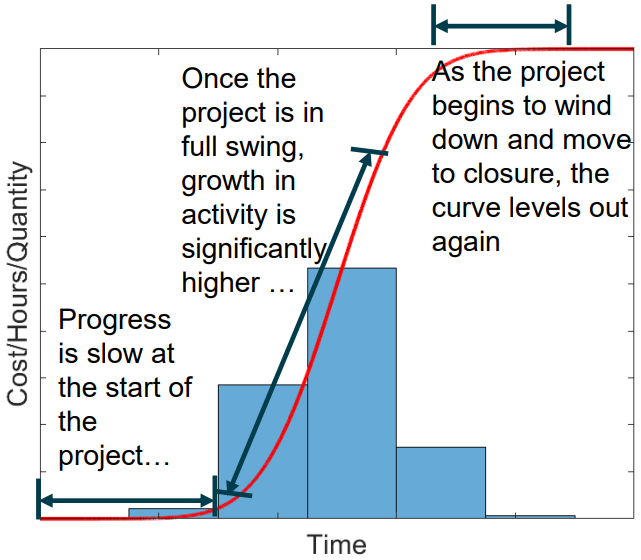
\includegraphics[width = 0.5\textwidth]{img/figure59.png}
    \caption{S-curve.}
\end{figure}
\subsection{What are s-curves used for?}
Resource allocation planning:
\begin{itemize}
    \item S-curves of expected person-hours versus time shows how the project team will need to flex over the project lifecycle
    \item This can aid the recruitment process
\end{itemize}
Project expenditure:
\begin{itemize}
    \item S-curves can show planned expenditure over the project time period
    \item If this is overlaid with information on when project funds are expected, cash flow problems can be identified
\end{itemize}
\subsection{Why are s-curves useful?}
S-curves can be used to compare real-time and projected progress.
\begin{figure}[H]
    \centering
    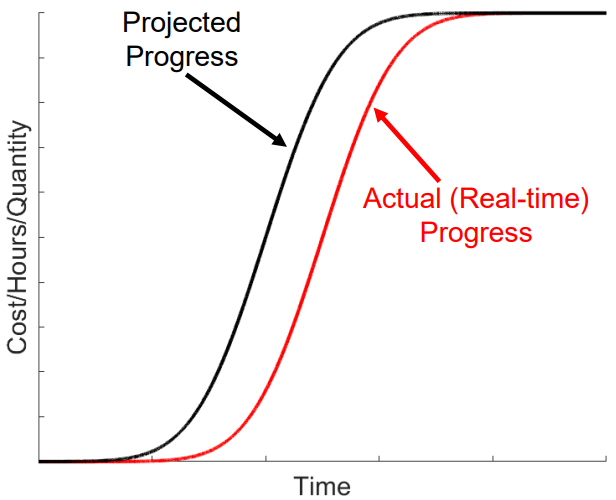
\includegraphics[width = 0.5\textwidth]{img/figure60.png}
    \caption{S-curve with real-time and projected progress.}
\end{figure}
\begin{itemize}
    \item S-curves help you to predict when resources will be heavily utilised
    \item S-curves help you manage stakeholder expectations
    \item S-curves help you plan for different schedule scenarios
\end{itemize}
\subsection{Example 6}
The ABC Corporation is planning a construction project with monthly projected receipts and expenditures as presented in the table below.
\begin{table}[H]
    \centering
    \small
    \setlength\tabcolsep{2pt}
    \begin{tabularx}{\textwidth}{@{}llllllllllllll@{}}
        \toprule
        \multicolumn{14}{l}{\textbf{ABC Corporation Construction Project}}                                                                                  \\
        \midrule
        Month                  & 1      & 2       & 3      & 4      & 5       & 6       & 7       & 8       & 9      & 10      & 11     & 12      & 13      \\
        Projected total        & 0      & 186,861 & 0      & 0      & 373723  & 0       & 0       & 0       & 0      & 934,307 & 0      & 186,861 & 186,861 \\
        receipts (\pounds)     &        &         &        &        &         &         &         &         &        &         &        &                   \\
        Projected total        & 30,000 & 114,338 & 50,000 & 40,062 & 110,396 & 200,000 & 200,000 & 441,535 & 55,215 & 55,675  & 40,000 & 40,000  & 0       \\
        expenditures (\pounds) &        &         &        &        &         &         &         &         &        &         &        &                   \\
        \bottomrule
    \end{tabularx}
    \caption{Example 6 table.}
\end{table}
\begin{figure}[H]
    \centering
    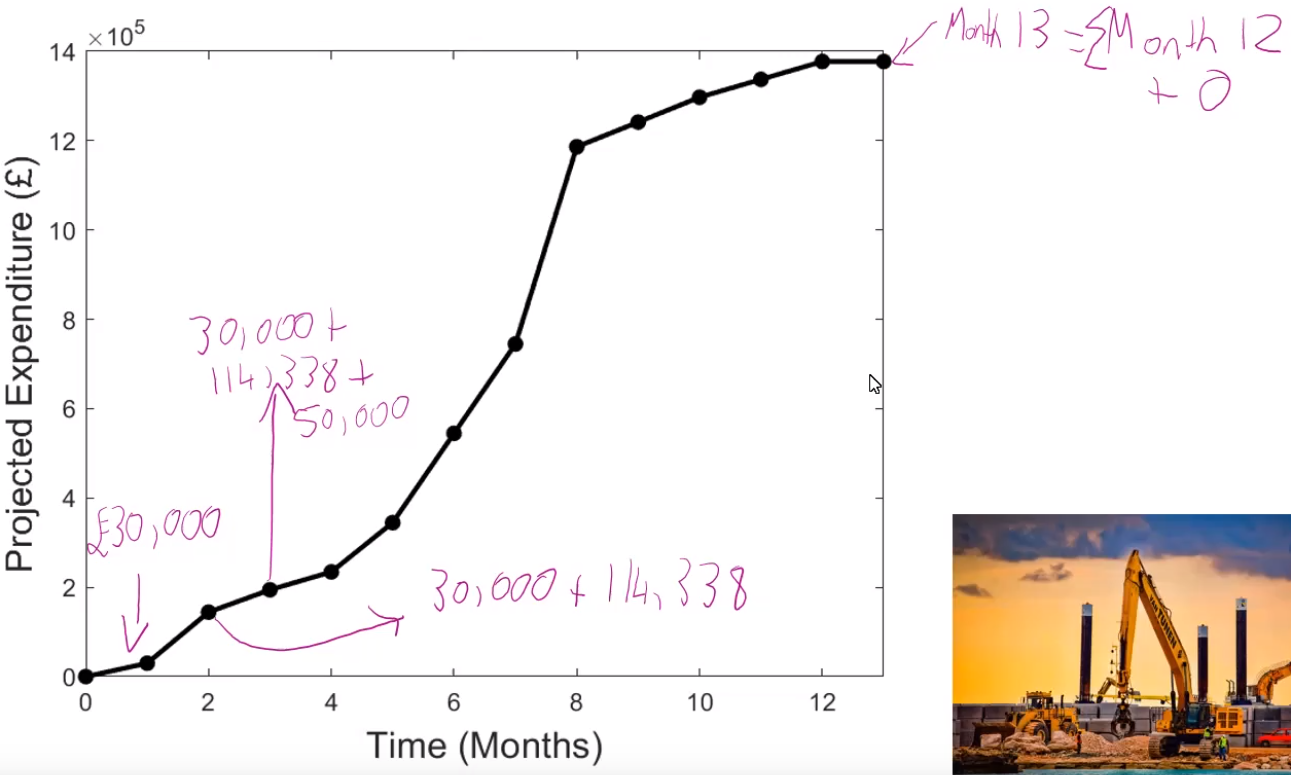
\includegraphics[width = 0.8\textwidth]{img/figure61.png}
    \caption{S-curve for example 6.}
\end{figure}
\begin{figure}[H]
    \centering
    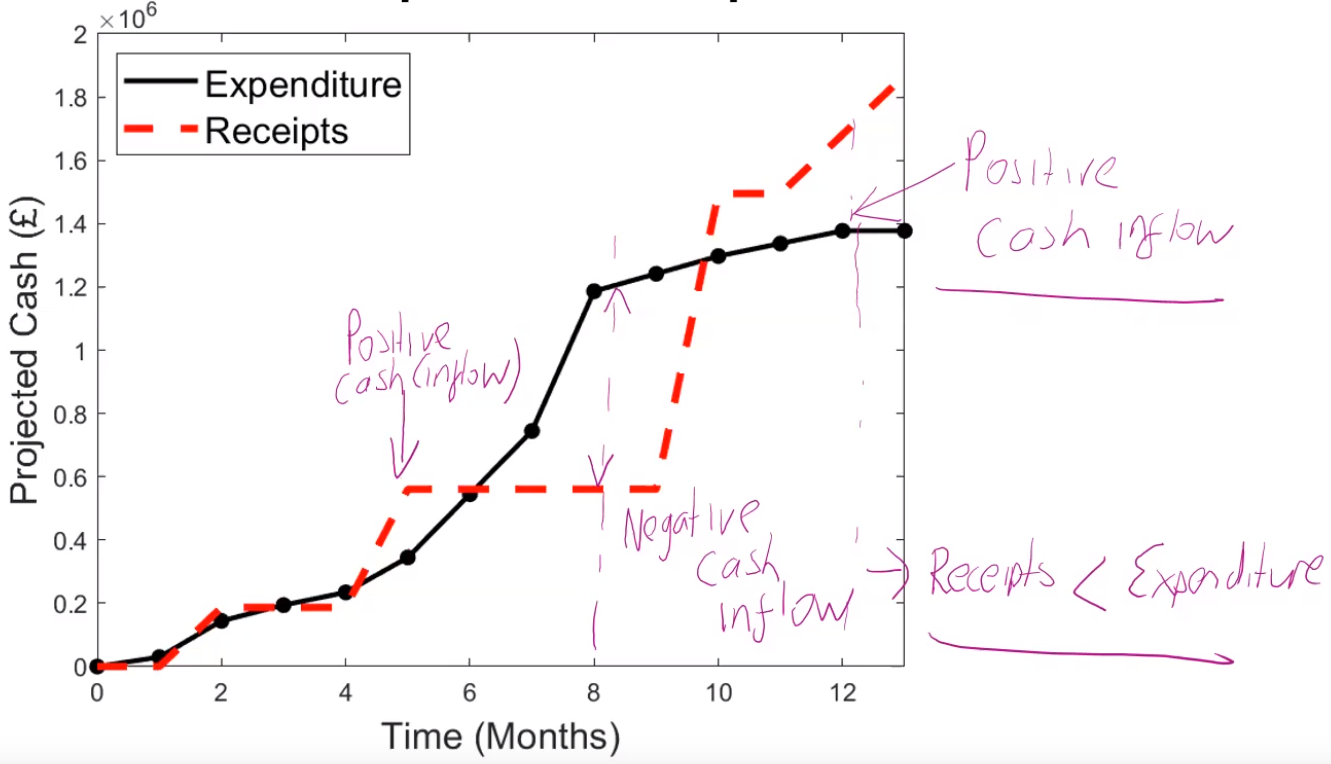
\includegraphics[width = 0.8\textwidth]{img/figure62.png}
    \caption{S-curve for example 6 with cash flow analysis.}
\end{figure}
\section{Summary}
\begin{itemize}
    \item Budgeting
          \begin{itemize}
              \item Definition of budgeting
              \item Description of budget types
              \item Demonstration of an operating budget
          \end{itemize}
    \item Cash flow forecasts
          \begin{itemize}
              \item Description of cash flow diagrams
              \item Description of cash flow tables
              \item Demonstrations of cash flow diagrams and tables
          \end{itemize}
    \item S-curves
          \begin{itemize}
              \item Description of s-curves
              \item Uses of s-curves
              \item Demonstration of constructing an s-curve for expenditure
          \end{itemize}
\end{itemize}